\documentclass[12pt]{texMemo} % originally by Rob Oakes; adapted by Alice Chen
%\usepackage{apa7}
\usepackage[style=apa, backend=biber]{biblatex}
\usepackage{graphicx}
\usepackage{csquotes,xpatch}
\usepackage{amsmath}

\DeclareCiteCommand{\citephoto}
{\boolfalse{citetracker}%
   \boolfalse{pagetracker}%
   \usebibmacro{prenote}}
{From "\printfield{title}," by \printnames[][-\value{listtotal}]{author}, \printdate, \printfield{journaltitle}, \printfield{volume}}
{\multicitedelim}
{\usebibmacro{postnote} (\printfield{doi})}

\defbibheading{shortbib}[References]{\subsubsection*{\centering #1}}
\addbibresource{Spoofing Project.bib}
\memoto{Navico: parent company of SIMRAD}
\memofrom{Joey Simone}
\memore{Recommendations for Development of Secure AIS in new SIMRAD AIS Transponders}
\memodate{15 April, 2024} % or \today
\memosection{NAU 420-1}

\begin{document}
\maketitle
Bottom Line Up Front: AIS Spoofing as a cyberattack is already in use by adversarial governments and maritime criminal enterprises the world over to alter or conceal information about ships, their business, their position, and the identities of the ships and the senders of AIS messages. The need for a secure AIS based on Public Key Cryptography is, at present, unfulfilled by the market. By spearheading the development of this technology, SIMRAD stands to not only save lives and enhance coastal law enforcement efforts but also gain a competitive edge in the market, particularly with the potential future mandates by the IMO and member nations. 




Addressing this issue is paramount. While efforts are underway to develop detection systems and algorithms to identify spoofed AIS data, transponder manufacturers possess a unique opportunity to combat spoofing at the software level. We can look to email cryptography for a path to follow. I have found a number of academic proposals for implementing Public Key Cryptography dating back to 2015, but each proposal has issues for backwards compatibility, time slots, amount of data being sent, or the ability to correlate a message with a signature. No solution has yet been implemented, but \textit{Securing the automatic identification system (AIS): using public key cryptography to prevent spoofing whilst retaining backwards compatibility} has analyzed the shortcomings by previous publications including by its own authors, and created the groundwork for a solution which should be workable by R\&D. Their solution solves the time slot problem, shields against replay attacks (Figure \ref{fig:replay}), provides a workflow for message verification, and uses VHF Data Exchange System (VDES) to solve the bandwidth problem \parencite[]{wimpenny_securing_2022}. The knowledge already exists, and PGP has existed in email for 30 years. 

Three things stand in the way of ending AIS spoofing. \begin{enumerate}
    \item Make AIS transponders which can send and receive signed messages and verify them. \footnote{Implement a way to shield access to the private key so malicious users can't copy a trusted key from a valid transponder into the memory of a spoofing transponder.}
    \item Coastal Governments install regulations pertaining to these cryptography enabled transponders and recommend or require them on ships needing Class A AIS. This may also come with the creation of a Certificate Authority\footnote{\begin{quote}
        [A Certificate Authority (CA)] which is a third party universally trusted by all users. The CA carries out checks as to the ownership of public keys and once satisfied that the public key belongs to the entity it reports to belong to, will digitally sign the public key, creating an attached ‘security certificate’. Any user would see the CA’s security certificate (the CA’s trusted digital signature) on a public key and will know that the public key is genuine and unmolested, assuming they have trust in the CA. \parencite[p 343]{wimpenny_securing_2022}
    \end{quote} }. This can be another kind of flag state control: if you trust the United States Coast Guard, you can trust this vessel's key.
    \item Registered vessels meeting the requirements of the regulation purchase and install Secure AIS transponders from the company, generate their private and public key pairs, have those keys signed by their flag state's CA, and sail confident in the information they receive from other ships and from AToNs and land stations.
\end{enumerate}

This will risk time, effort, and money to develop, but the problem is upon us, the framework exists, and if the company hesitates, another manufacturer will satisfy the market's need.
\newpage
\section*{Supplemental Information}
\begin{figure}[hb]
    \centering
    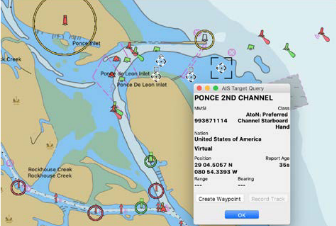
\includegraphics[width=0.5\linewidth]{bad-aton.png}
    \caption{AIS display of real and fake virtual AtoNs in Ponce De Leon Inlet, south of Daytona Beach, Florida. \citephoto[281]{kessler_protected_2020} CC BY-NC}
    \label{fig:Bad AToN}
\end{figure}
\begin{figure}[hb]
    \centering
    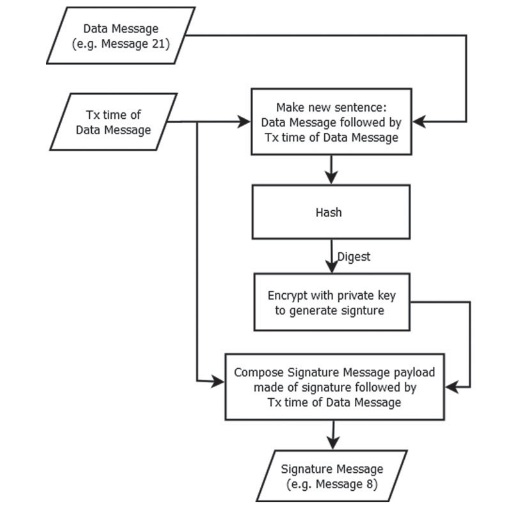
\includegraphics[width=.75\linewidth]{replay.png}
    \caption{Modified digital signing procedure to guard against replay attacks. \citephoto[p 338]{wimpenny_securing_2022} \copyright 2021 by \citeauthor{wimpenny_securing_2022}.}
    \label{fig:replay}
\end{figure}
\begin{figure}[hb]
    \centering
    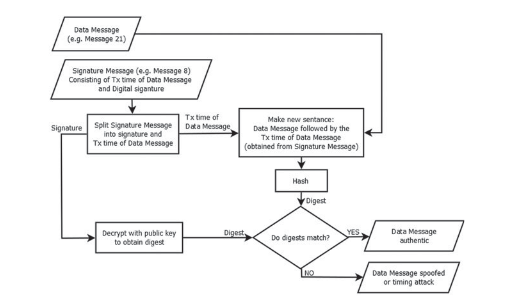
\includegraphics[width=0.75\linewidth]{verifiction.png}
    \caption{Verifying the Digital Signature. \citephoto[p 339]{wimpenny_securing_2022} \copyright 2021 by \citeauthor{wimpenny_securing_2022}.}
    \label{fig:verify}
\end{figure}
\begin{figure}[hb]
                \centering
                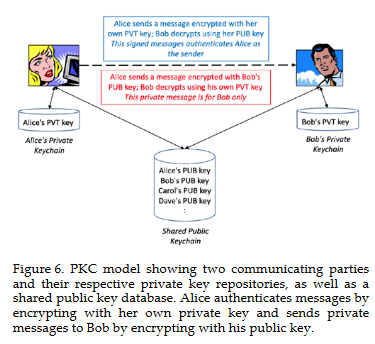
\includegraphics[width=0.5\linewidth]{AliceandBob.png}
                \caption{Alice and Bob are the frequently used examples in explanations of cryptography. \citephoto[282]{kessler_protected_2020} CC BY-NC}
                \label{fig:alice}
            \end{figure}
\clearpage
\printbibliography[heading=shortbib]
\newpage
\section*{Assessment of Sources}
\begin{enumerate}
    \item \citetitle*{androjna_ais_2024}
    \begin{enumerate}
    \item Explain why you chose the source or author and \emph{how it was useful}.
        \begin{itemize}
            \item This article makes the case for every aspect of the issue in one swoop, it is the before picture. A tanker concealing the illegal transfer of Russian Oil strikes the notes of Geopolitics, crime, and environmental issues in a single point. The article also lays out some of the ways that that data is manipulated, so it is good for itemized lists of possible AIS related cyber attacks.
        \end{itemize}
    \item Explain why the source or author has \emph{legitimate expertise} to weigh in on the topic.
        \begin{itemize}
            \item This author has written extensively on the subject, with 3 articles coming across my eyes in the early hours of research. Their job descriptions are also germane to the topic. Andrej Androjna and Marko Perkovič are in the Maritime Studies and Transportation faculty of the University of Ljubljana, Slovenia; Ivica Pavic is Faculty in Maritime Studies at the University of Split, Croatia, and Peter Vidmar is from the Department of Marine Traffic Engineering, Maritime University of Szczecin, Poland. I think that these titles imply a grasp on matters of navigation, global economy, and international strategy, especially with regards to Russia. They competently cite SOLAS and other treaties and regulations, and they have a very good grasp on the technical language as I, a junior American Mariner, understand, so I think that I can rely on them to tell me the half I don't get. The technical acumen and graphics from their AIS data are also stunning.
        \end{itemize}
    \item Identify and explain \emph{any bias that may exist} with this source or author.
        \begin{itemize}
            \item I'm gonna throw something at the wall and say that being a team composed of former eastern bloc countries that they have a bias against Russia. 
        \end{itemize}
\end{enumerate}
    \item \citetitle*{bateman_hms_2021}
    \begin{enumerate}
    \item Explain why you chose the source or author and \emph{how it was useful}.
        \begin{itemize}
            \item Ben actually picked this source, but it is the most dramatic occurrence of AIS spoofing, and the permanence of the Russia Ukraine War keeps the reference fresh in the mind. Nothing can drive home the importance of stopping spoofing like an attempt to use spoofing to actually start WWIII
        \end{itemize}
    \item Explain why the source or author has \emph{legitimate expertise} to weigh in on the topic.
        \begin{itemize}
            \item The author doesn't necessarily have expertise on cryptography or maritime affairs. However, he is a war reporter and State Department correspondent for the BBC, so I might say his expertise is in Geopolitics and Modern Conflict, which the article is mostly about.
        \end{itemize}
    \item Identify and explain \emph{any bias that may exist} with this source or author.
        \begin{itemize}
            \item It therefore follows that the lens he uses in the news article is that of the war reporter. The actions of ships and the equipment they use is irrelevant to him and the news team he writes for. His story is about Russia, and he calls it a war on reality. AIS Spoofing is just another tool that Crazy Ivan is using to prosecute their desperate violence, no different from a rifle in the hands of a foot soldier. 
        \end{itemize}
\end{enumerate}
 \item \citetitle*{kelly_novel_2022}
    \begin{enumerate}
    \item Explain why you chose the source or author and \emph{how it was useful}.
        \begin{itemize}
            \item The paper's introductory section has a good overview for the unfamiliar and uses layman's terms. Subsection 1.2 provides enough material for the entire "crime" heading of the Major Actors section of the project presentation. The paragraph \begin{quote}
                Vessels which are engaged in people trafficking or drug smuggling might attempt to obscure their position during a brief period when they are slowing down and then stopping, in order to exchange people or illegal cargo, with another vessel which also slows down. After the exchange is made both vessels resume normal AIS transmissions. Similarly, a vessel which has been involved in an accident with some maritime infrastructure such as warning buoys, or which has accidentally spilled oil, may immediately attempt to obscure or interfere with their AIS. Also, fishing vessels which are fishing in prohibited areas such as spawning grounds may try to obscure their AIS. \parencite[p 2]{kelly_novel_2022} 
            \end{quote} is remarkably clear. It also represents the current best technology we have for detecting spoofed data, without getting too bogged down with prevention of spoofing or with betting big on AI based detection schemes. It answers a question, "how can I detect a certain kind of lying by putting my investment in the Coast Guard
        \end{itemize}
    \item Explain why the source or author has \emph{legitimate expertise} to weigh in on the topic.
        \begin{itemize}
            \item The experiment is simple and looked sound to me, and although I don't understand the mathematics, the equations look juicy. Look at this from page 7
            \begin{equation*}
                P_R=G_RG_M \left(\frac{hB hM}{d^2}\right)^2\left(\frac{f}{40}\right)^2P_r
            \end{equation*} and tell me they're not experts \autocite{kelly_novel_2022}.
        \end{itemize}
    \item Identify and explain \emph{any bias that may exist} with this source or author.
        \begin{itemize}
            \item I think that this one might not have enough content for there to be a bias. He isn't even insisting that this is the right way, he just wants us to check out this cool thing he figured out. Maybe the bias lies in the introductory section and the fact that he chooses human and drug trafficking before illegal fishing demonstrates that he cares more about humans and drugs than fish, but I think this is a pretty uncontroversial bias to have outside of Atlantis.
        \end{itemize}
\end{enumerate}
 \item \citetitle*{kessler_protected_2020}
    \begin{enumerate}
    \item Explain why you chose the source or author and \emph{how it was useful}.
        \begin{itemize}
            \item This is one of a few articles that came up on the library search when I wanted to find out if someone had already made the paper that I wanted to write when Ben recommended the subject. I figured that "demonstration" means that he made a working prototype, and that the solution that appealed to my nerdy sensibilities was not a pipe dream. The abstract is the premise of this memo. \begin{quote}
                The Automatic Identification System (AIS) provides situational awareness for vessels at sea. AIS has a number of known security vulnerabilities that can lead to a several types of attacks on AIS, including the ability to create ghost vessels, false warning or meteorological messages, or bogus virtual aids-to-navigation (AtoN). A number of methods, with varying levels of complexity, have been proposed to better secure AIS and, indeed, emerging AIS protocols will implement some of these mechanisms. Nevertheless, little has been done to secure the current standards, which will remain in use for some time. This paper presents Protected AIS (pAIS), a demonstration of capability implementation using public-key cryptography methods to address several AIS security vulnerabilities, maintain backward compatibility, and be able to interoperate with non-pAIS devices. \parencite[279]{kessler_protected_2020}
            \end{quote}
        \end{itemize}
    \item Explain why the source or author has \emph{legitimate expertise} to weigh in on the topic.
        \begin{itemize}
            \item It's the Journal of Marine Navigation! If anything, I want to get published in it for writing something cool. The articles approved for publishing in this journal have to be by subject matter expert deckies, so they would have the most complete understanding of the marine operations part of the concept. The graphics also have important nods to traditions of cryptography which are also dear to me (Figure \ref{fig:alice}). 
            
        \end{itemize}
    \item Identify and explain \emph{any bias that may exist} with this source or author.
        \begin{itemize}
            \item Perhaps revealed in the end of the conclusion on 285, Kessler essentially denies the utility of his entire proof-of-concept by saying "[pAIS]  will ultimately do little good because bad actors will continue to operate in the non-secure mode and others will accept their messages. Without a strong policy that requires use of secure methods, add-on security will not achieve the goal of a secure AIS network." \autocite{kessler_protected_2020}. His bias may be that the technology is all well and good but useless without the force of the law to make the secure mode mandatory.
        \end{itemize}
\end{enumerate}
 \item \citetitle*{wimpenny_securing_2022}
    \begin{enumerate}
    \item Explain why you chose the source or author and \emph{how it was useful}.
        \begin{itemize}
            \item This source is essentially the article I wanted to write. I had suspected early into the project that cryptography was the best solution to AIS spoofing, in part because of my own familiarity with the encryption technology as it applies to email security. Whereas usually when encryption and PGP are broached in conversations about email, the focus is on keeping unauthorized parties from reading the contents of a message, and verification of the sender is a convenient bonus, in AIS security, it's important that everyone can read a message, but AIS has no way of verifying a sender. I used to cryptographically sign my emails, because nobody I knew used PGP for email security, so I couldn't send or receive encrypted messages, but people who knew how to use the software and who had trusted someone who has trusted my key could be sure it was me sending the message. I was also a crypto-bro in my years spent as a teenage boy, so when some of the digital banks and crypto exchanges started signing their messages, I was just excited to be able to use the skill, and at one point I actually was able to detect a phishing attack because a legitimate looking email had a bad signature. Using the Wimpenny article, I can gain credibility by inserting what I was already going to say as quotes. Not to mention the backwards compatibility being a huge selling point. It is much easier to swallow a change when not all the industry in the whole world need change at the same time.
        \end{itemize}
    \item Explain why the source or author has \emph{legitimate expertise} to weigh in on the topic.
        \begin{itemize}
            \item They show a good understanding of the existing technology, their descriptions of the GMDSS equipment and protocols align with and exceed my current understanding; a good sign considering I'm not dumb. The same authors have been cited by some of the other papers I read while constructing my understanding of the topic as a whole, including themselves. I have read their 2018 article "Public Key Authentication for AIS and the VHF Data Exchange System (VDES)." in \textit{Proceedings of the 31st International Technical Meeting of the Satellite Division of The Institute of Navigation} and was similarly satisfied with their knowledge of security and cryptography. These authors are some of the only people in the sphere talking about this, the others cite them and they all cite each other, which sounds like a peer review with extra steps.
        \end{itemize}
    \item Identify and explain \emph{any bias that may exist} with this source or author.
        \begin{itemize}
            \item Their bias is the same as mine, for much the reason I've described. Gareth Wimpenny has his name on about 8 articles that are pretty similar to each other and to mine, this is certainly enough to get stuck in one's ways. Most of their sources are my sources too. 
        \end{itemize}
\end{enumerate}
\end{enumerate}

\end{document}